%!TEX root = ../template.tex
%%%%%%%%%%%%%%%%%%%%%%%%%%%%%%%%%%%%%%%%%%%%%%%%%%%%%%%%%%%%%%%%%%%%
%% chapter4.tex
%% NOVA thesis document file
%%
%% Chapter with lots of dummy text
%%%%%%%%%%%%%%%%%%%%%%%%%%%%%%%%%%%%%%%%%%%%%%%%%%%%%%%%%%%%%%%%%%%%

\typeout{NT FILE chapter4.tex}%

\chapter{From Biprograms to OCaml -- Methodology and Tool}
\label{cha:methodology}


\FloatBarrier
\section{From WhyRel to bip2ml}
\label{sec:whyrel_to_bip2ml}

WhyRel describes a pratical approach to the verification of program equivalence based on product programs.
It also provides a set of \hyperref[fig:translation-biprograms-rules]{rules} that guides the translation, in the case of WhyRel, from the biprograms language to WhyML.
Its authors deeply explore the problems that pointer based programs bring to the table, but this is not an objetive of this thesis.
Instead, we defined and formalized a programming language called $BipLang$.
BipLang's main purpose is writing biprograms and was based on the biprograms language used in WhyRel's work.
BipLang was designed to accept Gospel annotations and to be as similar as possible to OCaml in terms of syntax and semantics.
We did that in order to allow programmers that are used to that language to verify the equivalence of their programs without needing to learn a new language or completely rewrite their code or specification.
Then, we transpile the biprograms using the translation rules defined by WhyRel's authors to produce Gospel-annotated OCaml code.


\FloatBarrier
\section{bip2ml}
\label{sec:bip2ml}

\FloatBarrier
\subsection{Overview and Architecture}
\label{subsec:bip2ml_overview}

$bip2ml$ is a transpiler that takes Gospel-annotated BipLang code and outputs Gospel-annotated OCaml code.
This tool brings the contributions of WhyRel into the world of OCaml, Gospel and Cameleer.
All of the work done on this thesis is available at \url{https://github.com/JoaoNini75/MasterThesis}, which includes bip2ml's code, this thesis' LateX code and other related material.

We now describe bip2ml's pipeline and how it \hyperref[fig:bip2ml_cameleer_pipeline]{integrates} with Cameleer.
The users are expected to start with two programs and aim to formally verify that they are equivalent.
There may be some exceptions to this that we will discuss later in the \hyperref[cha:case_studies]{case studies} chapter, but this is our starting point and main objective.
The first step requires the user to provide the alignment of the two unary programs, writing a BipLang program with the necessary Gospel annotations.
After that, the user feeds bip2ml that .bip file and it starts its work to produce the OCaml + Gospel program.
The transpiler's output file can then be fed to Cameleer, which in turn will take care of the rest of the verification process, exactly as if we gave it an OCaml program that we wrote manually.

\begin{figure}[htbp]
  \centering
  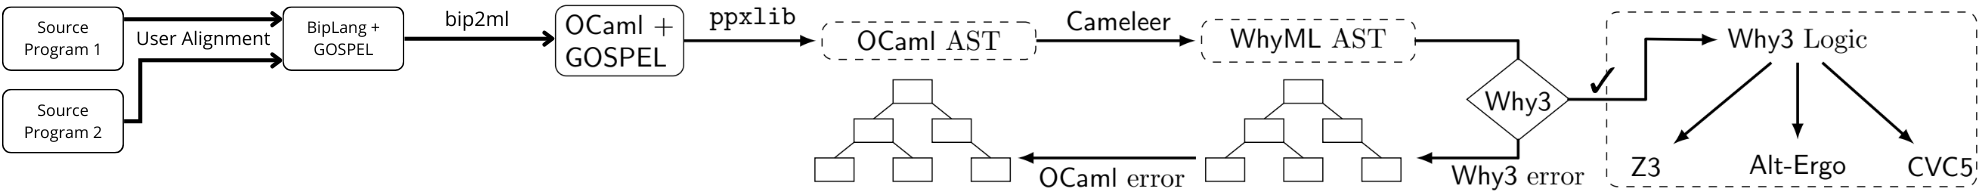
\includegraphics[max width=\textwidth]{bip2ml+cameleer_pipeline}
  \caption{Architecture and verification pipeline of bip2ml and Cameleer.}
  \label{fig:bip2ml_cameleer_pipeline}
\end{figure}

The bip2ml transpiler is itself also a \hyperref[fig:bip2ml_cameleer_pipeline]{pipeline}, that takes the input through four phases / components before terminating.
The first component is the lexer, which defines what are the keywords and tokens accepted by BipLang; if any error occurs during this phase, bip2ml outputs \emph{"lexical error"} to the terminal.
We used ocamllex~\cite{ocamllex} to develop our lexer.
Representing the second part of the transpiler, we have the parser, that takes the lexer's output and, by comparing it with the rules we define that are valid BipLang constructions, determines if the source code's structure is valid or not.
If it is not, it outputs \emph{"syntax error"} to the terminal.
To program the parser, we utilized Menhir~\cite{menhir}.
The output of the parser is an AST, the BipLang AST, which is the input of the next phase: the translator.
This component is the one responsible for translating the BipLang AST into the OCaml AST, according to the 8 rules defined by WhyRel; this phase does not fail.
Finally, we named the last part of our transpiler the printer, since its function is to receive the OCaml AST from the translator and outputting to the terminal or to a file the final OCaml code with all the Gospel specifications.
Both the translator and the printer were implemented using OCaml directly.

\begin{figure}[htbp]
  \centering
  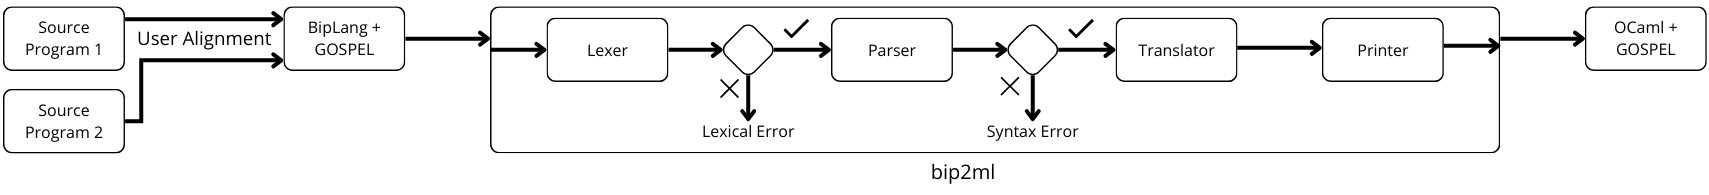
\includegraphics[max width=\textwidth]{bip2ml_pipeline}
  \caption{Architecture and pipeline of bip2ml.}
  \label{fig:bip2ml_pipeline}
\end{figure}

bip2ml was tested with several examples that were separated into different files depending on the features they target.
These tests were automated using Dune~\cite{dune}.

We also developed a VSCode extension that provides syntax highlighting for BipLang.
Although it is dispensable, it certainly was extremely helpful during the whole development and testing of bip2ml, and it may also be a relevant aid to anyone that programs in BipLang.
It was heavily based on OCaml Labs' VSCode OCaml Platform~\cite{ocaml-platform}, since the syntaxes of OCaml and BipLang are nearly identical.


\FloatBarrier
\subsection{BipLang: language definition}
\label{subsec:lang_def}

BipLang's syntax, semantics and AST are very similar to OCaml's.
Although BipLang implements the most common OCaml language constructions, there are definitely some missing, such as exceptions and object-oriented features.
Taking that into consideration, it is also important to remember that, regarding the scope of this thesis, these constructions can not be seen as very relevant.
On the other hand, our language adds 3 constructions that are not present in OCaml: the pipe, the floors and the conditionally aligned loops.
Their semantics are the same as in WhyRel's work.

We now present the grammar of our language, BipLang.
The syntaxes of the most relevant rules are given by the following extended BNF definition.
Note that Biplang's keywords are written in orange.

\begin{lstlisting}[mathescape, basicstyle=\ttfamily, columns=flexible,
                    emph={type, and, let, rec, if, then, else, mod, in, for, while, do, done, to, begin, end, assert, match, with, of, open, include,ref},
                    emphstyle=\ttfamily\bfseries\color{myorange}]
file ::= decl*

decl ::= 
            | def
            | spec
            | typedef

spec ::= { loc: location; text: string; }

typedef ::=
              | type id = payload (and typedef)?
              | type id = $\overrightarrow{constructor}$ (and typedef)?

payload ::= 
              | $\overrightarrow{bt}$
              | $\overrightarrow{id}$

constructor ::= idc * payload?

def ::= let rec? id ($\overrightarrow{parameter}$) : fun_ret? = $\overrightarrow{expr}$ spec

expr ::=
            | ()
            | (e)
            | c
            | id
            | -e
            | $\neg$ e
            | ref e 
            | !e
            | e + e
            | e - e
            | e * e
            | e / e
            | e mod e
            | e = e
            | e <> e
            | e < e
            | e $\leq$ e
            | e > e
            | e $\geq$ e
            | e == e
            | e != e
            | e && e
            | e || e 
            | e ^ e
            | let id = e in $\overrightarrow{e}$
            | if e then e else e
            | for id = e to e do spec? e done 
            | while e do spec? e done 
            | id := e
            | assert (e)
            | match id with ($\overrightarrow{case}$)
            | ($\overrightarrow{e}$)
            | idc ($\overrightarrow{e}$)
            | fun_name ($\overrightarrow{e}$)
            | Module_name.fun_name ($\overrightarrow{e}$)
            | def in e
            
            $\emph{arrays}$
            | [| $\overrightarrow{e}$ |]
            | id.(e)
            | id.(e) <- e

            $\emph{lists}$
            | [ $\overrightarrow{e}$ ]
            | e :: [ $\overrightarrow{e}$ ]
            | e @ [ $\overrightarrow{e}$ ]

            $\emph{introduced by BipLang}$
            | e <|> e $\emph{(pipe)}$
            | $\lfloor e \rfloor$ $\emph{(floors)}$
            | while e <|> e . e <|> e do spec? e done
            $\emph{(conditionally aligned loops)}$

c ::=
        | None
        | int
        | bool
        | string

\end{lstlisting}

We simplified some things for the sake of readibility and there are some omissions in the grammar, which we will explain now.
Firstly, we use $c$ to simply represent a constant.
Additionally, notice that we use $id$ and $idc$.
They both refer to identifiers but $id$ refers to an all lowercase identifier, while $idc$ stands for "capitalized id", so its first letter is capital.
This is important to distinguish since module calls and type constructors, for example, use capitalized names, but lowercase identifiers are the standard for the names of variables and functions, among others.
Next, we have to show the difference between $bt$ (bip type) and $at$ (any type).
$bt$ represents the basic types (bool, int, string, none), but $at$ extends that definition to also allow $id$.
This is useful, for example, when we have a parameter of a user-defined type:

\begin{lstlisting}[mathescape, basicstyle=\ttfamily, columns=flexible,
                    emph={type, and, let, rec, if, then, else, mod, in, for, while, do, done, to, begin, end, assert, match, with, of, open, include,ref},
                    emphstyle=\ttfamily\bfseries\color{myorange}]
type advanced_number = 
	| Pos of int
	| Neg of int
	| Zero

let example (an : advanced_number) : advanced_number = begin
	(...)
end
\end{lstlisting}

Otherwise, we would be limited to parameters and function returns of the basic types ($bt$).
$parameter$ is pretty straightforward: it represents a parameter, with all its possible variations, having pipe, floors or none, explicitly saying its type or not.
$fun\_ret$ is optional and represents what the function returns, allowing explicit or implicit type definition and also pipe, floors or none of them.
$constructor$ represents the definition of a constructor within a type defintion and $payload$ represents a type definition that has no constructors:

\begin{lstlisting}[mathescape, basicstyle=\ttfamily, columns=flexible,
                    emph={type, and, let, rec, if, then, else, mod, in, for, while, do, done, to, begin, end, assert, match, with, of, open, include,ref},
                    emphstyle=\ttfamily\bfseries\color{myorange}]
type constructors_example = 
	| Pos of int
	| Neg of int
	| Zero

type payload_example = int * bool * string
\end{lstlisting}

$case$ represents a case of the \emph{match...with} construction when we do pattern matching.
It is constituted by two parts, a pattern and an expression.
The pattern represents the structure that each case will compare against the "parameter" of the \emph{match...with} constructor, i.e, the left side of the arrow.
The expression corresponds to what gets executed if a given case is the chosen one, i.e, the right side of the arrow:

\begin{lstlisting}[mathescape, basicstyle=\ttfamily, columns=flexible,
                    emph={type, and, let, rec, if, then, else, mod, in, for, while, do, done, to, begin, end, assert, match, with, of, open, include,ref},
                    emphstyle=\ttfamily\bfseries\color{myorange}]
let case_example (x : int) : int = begin
  match x with
  | 0 -> 10
  | 1 -> 11
  | _ -> -1 
end
\end{lstlisting}


\FloatBarrier
\subsection{Translator and Printer}
\label{subsec:translator_printer}

\subsubsection{Design Choices and Implementation Details}
\label{subsubsec:translator_printer_details}

Before we demonstrate how our translator and printer work by applying WhyRel's translation \hyperref[fig:translation-biprograms-rules]{rules}, there are some details about our printer that we want to make clear.
Adding $\_l$ to the left side program and $\_r$ to the right side program was a printing choice that could be changed to anything the reader prefers when identifying to what program a given identifier belongs to.
Additionally, it is relevant to mention that the output code you will read below was not formatted manually to be easier to read; it was only adjusted to fit the page.
bip2ml effectively prints OCaml code respecting general good indentation practices.
The choice of using two whitespaces for the indentation is also something that can easily change by simply setting a variable in our printer to a different value.

As a way to make the Gospel specifications coherent with the generated OCaml code and make sure which variable the user refers to, we require the user to write the specification using $\_l$ when reasoning about the left side and $\_r$ for the right side.
Additionally, as a parser design choice, we also require that each function has a Gospel specification immediately after its declaration.
If you do not want to write the specification in a given moment but want bip2ml to execute without a parsing error, you can simply do the following:
\begin{lstlisting}[mathescape, basicstyle=\ttfamily, columns=flexible,
                    emph={type, and, let, rec, if, then, else, mod, in, for, while, do, done, to, begin, end, assert, match, with, of, open, include,ref},
                    emphstyle=\ttfamily\bfseries\color{myorange}]
let your_function () = begin
  (your code...)
end
(*@*)
\end{lstlisting}


\subsubsection{Demonstrating translation through examples}
\label{subsubsec:translator_printer_examples}

We now present 3 examples: the first applies rules 1, 2, 3 and 5, the second showcases rules 4, 6 and 7 and the third demonstrates rule 8.
Note that we use, in our transpiler, the rules exactly as the authors of WhyRel defined them. 
We will omit the necessary Gospel specifications to prove these examples, since it is not our focus in this subsection.
Notice that the names of the functions are different depending if they belong to the input or output; bip2ml does not apply this renaming, we did it to avoid confusion.

\begin{figure}[h]
  \centering

  \begin{subfigure}[t]{0.49\textwidth}
    \centering
    \noindent
    \begin{biplangenv}


let invert_bip (x : int) = begin
  -x
end

let triple_bip (|_ s : string _|,
  n) = begin
  |_ s ^ s ^ s _|
end

let first_bip () = begin
  let number = 1 <|> 1 in
  let message = |_ "Hello" _| in
  let app_res = invert_bip (3) in
  let triple_res = |_ triple_bip
    (message, number) _| in
  message <|> message
end
    \end{biplangenv}
  \end{subfigure}
  \hfill
  \begin{subfigure}[t]{0.49\textwidth}
    \centering
    \noindent
    \begin{gospel}


let invert_ocaml (x : int) =
  -x

let triple_ocaml (s_l : string)
  (s_r : string) (n_l) (n_r) =
  (((s_l ^ s_l) ^ s_l),
   ((s_r ^ s_r) ^ s_r))

let first_ocaml () =
  let number_l = 1 in
  let number_r = 1 in
  let message_l = "Hello" in
  let message_r = "Hello" in
  let app_res = invert_bip (3) in
  let triple_res = triple_bip
    (message_l) (message_r)
    (number_l) (number_r) in
  (message_l, message_r)
    \end{gospel}
  \end{subfigure}
  \caption{Translation example for rules 1, 2, 3 and 5.}
  \label{fig:trans_ex_first}
\end{figure}

The first line of code of \hyperref[fig:trans_ex_first]{$first\_bip$}, \emph{let number = 1 <|> 1 in}, uses rule 5 to rename the variables declared inside a $let...in$, with the same identifier and separated by a pipe.
Therefore, in the OCaml version, we get the lines \emph{let number\_l = 1 in let number\_r = 1 in}.

The next line, \emph{let message = |\_ "Hello" \_| in}, makes use of rule number 3 to translate the expression inside the floors into a pipe with two equal expressions on each side.
This shows that every floor is a pipe, but not every pipe can be a floor.
This happens because if we have $C_1 | C_2$ and $C_1 \neq C_2$, we cannot "compress" the pipe into a floored expression; otherwise, with $C_1 = C_2$, we would be able to establish that $C_1 | C_2$ is the same as $\lfloor C_1 \rfloor$.
So, bip2ml internally translates the original line to \emph{let message = "Hello" <|> "Hello" in} and finally outputs \emph{let message\_l = "Hello" in let message\_r = "Hello" in}, as we can see in the OCaml code.

The third line of $first\_bip$ is a binding to a function call: \emph{let res = invert\_bip (3) in}.
In this case, no rule is being used since the function call is not inside floors, therefore the input and output are the same.
However, in the next line, \emph{let triple\_res = |\_ triple\_bip (message, number) \_| in}, that is the case, so rule 2 is applied here.
This rule interpolates the arguments of the function call so that we get the first argument for the left side, then that same argument for the right side, and all the other possible other ones, respecting the order defined in the biprogram and interpolating the left and right sides.
So, we get the output \emph{let triple\_res = triple\_bip (message\_l) (message\_r) (number\_l) (number\_r) in}.

Finally, in the last line of $first\_bip$, \emph{message <|> message}, we utilized rule 1, which translates two expressions separated by a pipe into two sequential expressions in general.
In this particular case, however, since this is the value returned by the function, it returns them as a binary tuple, with the adequate identifier renaming: \emph{(message\_l, message\_r)}.

\begin{figure}[h]
  \centering

  \begin{subfigure}[t]{0.49\textwidth}
    \centering
    \noindent
    \begin{biplangenv}

      
let second_bip (|_c : bool _|,
  n : int) : |_int_| = begin

  if |_c_| 
  then begin |_1_| end
  else begin 
    let i = |_ ref 0 _| in
    let res = |_ ref 0 _| in

    while |_ !i < n _| do
      i := |_ !i + 1 _|;
      res := |_ !res * !i _|
    done;

    |_ !res _|
  end
end
    \end{biplangenv}
  \end{subfigure}
  \hfill
  \begin{subfigure}[t]{0.49\textwidth}
    \centering
    \noindent
    \begin{gospel}


let second_ocaml (c_l : bool)
  (c_r : bool) (n_l : int)
  (n_r : int) : int * int =

  assert ( (c_l) = (c_r) );
  if c_l
  then begin 
    (1, 1)
  end else begin 
    let i_l = ref (0) in
    let i_r = ref (0) in
    let res_l = ref (0) in
    let res_r = ref (0) in

    while (!i_l < n_l) do
      (*@ invariant ((!i_l < n_l)) 
                 <-> ((!i_r < n_r))*)
      i_l := (!i_l + 1);
      i_r := (!i_r + 1);
      res_l := (!res_l * !i_l);
      res_r := (!res_r * !i_r)
    done;

    (!res_l, !res_r)
  end
    \end{gospel}
  \end{subfigure}
  \caption{Translation example for rules 4, 6 and 7.}
  \label{fig:trans-ex-second}
\end{figure}

Moving on to the \hyperref[fig:trans-ex-second]{second} example, attent to the use of floors in the parameters and on the type returned by the $second\_bip$ function.
The first statements indicate the use of an \emph{if...then...else} block of code, which is translated by rule 6.
Firstly, the rule introduces an assertion that makes the program fail during its execution if the condition is not evaluated equally in both sides.
After that, we use one of the conditions, in this case, WhyRel authors chose the left side one, but we could use the right side condition, since we just established that they are equal.
The \emph{then} and \emph{else} branches will then get recursively translated, so we get this translated code: \emph{assert ( (c\_l) = (c\_r) ); if c\_l then begin (...) end else begin (...) end}. 
The \emph{if} branch's translation is done by using rule 3 and then rule 1, returning that constant for both programs as a binary tuple: \emph{(1, 1)}.
Next, inside the \emph{else} there is a while loop, which is translated following rule number 7.
Similarly to the \emph{if...then...else} block, we ignore the right side condition and use the left side one to limit the loop execution.
However, contrary to the assertion used in rule 6, here a loop invariant is added so we guarantee that the condition on both sides is always evaluated to the same value during the whole execution of the \emph{while}.
The body of the cycle will then get recursively translated, which gets us the following translated code (and specification): \emph{while (!i\_l < n\_l) do (*@ invariant ((!i\_l < n\_l)) <-> ((!i\_r < n\_r))*) (...) done}.
Finally, we get to see rule 4 applied to the statements inside the while loop, translating sequential BipLang instructions to sequential OCaml instructions, applying the necessary transformations to those statements individually.
The code lines we are mentioning are these: \emph{i := |\_ !i + 1 \_|; res := |\_ !res * !i \_|}.
In practice, there is not a visual outcome of this rule, but, since we are here applying rule 3 too, the output looks like this: \emph{i\_l := (!i\_l + 1); i\_r := (!i\_r + 1); res\_l := (!res\_l * !i\_l); res\_r := (!res\_r * !i\_r)}.

\begin{figure}[h]
  \centering

  \begin{subfigure}[t]{\textwidth}
    \noindent
    \begin{biplangenv}


let counting_bip (|_ target : int _|, |_ mult_of _|) : |_ int _| = begin
  let counter = |_ ref 0 _| in

  while (!counter < target) <|> (!counter < target) .
        (!counter mod mult_of = 0) <|> (!counter mod mult_of = 0) do
    counter := |_ !counter + 1 _|
  done;

  |_ !counter _|
end
    \end{biplangenv}
  \end{subfigure}
  \hfill
  \begin{subfigure}[t]{\textwidth}
    \centering
    \noindent
    \begin{gospel}


let counting_ocaml (target_l : int) (target_r : int) (mult_of_l)
  (mult_of_r) : int * int =

  let counter_l = ref (0) in
  let counter_r = ref (0) in

  while ((!counter_l < target_l) || (!counter_r < target_r)) do
    (*@ invariant  
      (!counter_l < target_l && mod !counter_l mult_of_l = 0) ||
      (!counter_r < target_r && mod !counter_r mult_of_r = 0) ||
      (not (!counter_l < target_l) && not (!counter_r < target_r)) ||
      (!counter_l < target_l && !counter_r < target_r) *)
    
    if ((!counter_l < target_l) && ((!counter_l mod mult_of_l) = 0))
    then begin 
      counter_l := (!counter_l + 1)
    end else begin 
      if ((!counter_r < target_r) && ((!counter_r mod mult_of_r) = 0))
      then begin 
        counter_r := (!counter_r + 1)
      end else begin 
        counter_l := (!counter_l + 1);
        counter_r := (!counter_r + 1)
      end
    end
  done;

  (!counter_l, !counter_r)
    \end{gospel}
  \end{subfigure}
  \caption{Translation example for rule 8.}
  \label{fig:trans-ex-third}
\end{figure}

Let us look now at the \hyperref[fig:trans-ex-third]{third} and last example.
This one showcases the use of rule 8, that translates conditionally aligned loops.
This rules takes as input a while loop with two alignment guards and outputs a while loop with a transformed body and a rather complex invariant, $A$.

$A$ corresponds to the logical disjunction of 4 main formulas, that are all a conjunction themselves.
The first represents the left loop condition \emph{and} the left alignment guard.
The second conjunction is the same but for the right side.
The third corresponds to the conjunction of the negated loop conditions.
The final conjunction is the same as the previous one but with the original loop conditions.

The generated invariant's structure is defined by the rule, varying only in the values that each expression is evaluated to.
Nevertheless, our transpiler allows the user to add Gospel specifications to the original while loop and those reasonings will be copied and put together with the automatically generated $A$ invariant, appearing in the output.

The body becomes a \emph{if...then...else if...then...else} block, so there are three possible outcomes for each iteration of the cycle.
The first occurs when the loop condition for the left program and the left alignment guard are both evaluated to true, therefore executing only the instructions that refer to the left side.
The second branch works in a very similar way to the previous, but applied to the right side program.
The third case happens when the loop condition (on the left side) is respected but none of the alignment guards are, resulting in the execution of all the instructions inside the original biprogram's cycle.

